\documentclass[border=2mm,12pt]{standalone}
\usepackage{fouriernc}
\usepackage{tikz}
\usepackage{tkz-euclide}

\usetikzlibrary{shadings}
\begin{document}
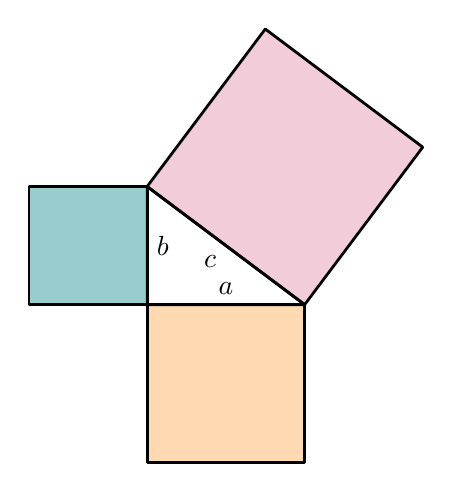
\begin{tikzpicture}[scale=.5]
\tkzDefPoint(0,0){C} \tkzDefPoint(4,0){A}
\tkzDefPoint(0,3){B}
\tkzDefSquare(B,A)
\tkzGetPoints{E}{F}
\tkzDefSquare(A,C)
\tkzGetPoints{G}{H}
\tkzDefSquare(C,B)
\tkzGetPoints{I}{J}
\tkzFillPolygon[color = orange!30
](A,C,G,H)
\tkzFillPolygon[color = teal!40 ](C,B,I,J)
\tkzFillPolygon[color = purple!20](B,A,E,F)
\tkzDrawPolygon[line width = 1pt](A,B,C)
\tkzDrawPolygon[line width = 1pt](A,C,G,H)
\tkzDrawPolygon[line width = 1pt](C,B,I,J)
\tkzDrawPolygon[line width = 1pt](B,A,E,F)
\tkzLabelSegment[above](C,A){$a$}
\tkzLabelSegment[right](B,C){$b$}
\tkzLabelSegment[below left](B,A){$c$}
\end{tikzpicture}
\end{document}